\documentclass{article}
\usepackage[utf8]{inputenc}
\usepackage[T1]{fontenc}
\usepackage{lmodern}
\usepackage{graphicx}
\usepackage[frenchb]{babel}
\usepackage{hyperref}
\usepackage[table,xcdraw]{xcolor}
\usepackage{float}

\newcommand{\info}{\texttt}
\newcommand{\pattern}{\emph}
\newcommand{\ue}{\textbf{X5I0010 "Objet et développement d'applications"}}

\title{Objet et développement d'applications - Design Patterns\\
Projet libre : BloodBowl}
\author{Elbert Noel \bsc{NYUNTING} \and Corentin \bsc{CHÉDOTAL}}
\date{19 Novembre 2016}

%PEUT ETRE CHANGER LES MARGES DU DOCUMENT POUR AVOIR PLUS DE PLACE

\begin{document}

\maketitle

\centerline{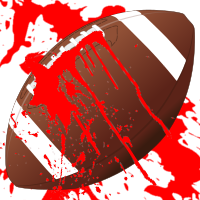
\includegraphics[scale=0.75]{img/logo.png}}

\begin{abstract}
    Dans le cadre de l'UE X5I0010 "Objet et développement d'applications" nous avons réalisé ce projet. Il comporte comme demandé plusieurs "designs patterns". Ont été utilisé les patterns \pattern{Strategy}, \pattern{State}, \pattern{Command}, \pattern{Abstract Factory}. Ce rapport expliquera leur implémentation, le but et fonctionnement du projet ainsi que les difficultés rencontrées dans la réalisation de celui-ci.
\end{abstract}

\tableofcontents

\section{Introduction}
    
    L'Unité d'Enseignement \ue requérait la réalisation d'un projet de fin de semestre. Nous avions carte blanche dans le choix du sujet du projet (dans les limites du raisonnable bien sur). Notre binôme ayant un fort intérêt pour les jeux vidéos nous avons très tôt décidé de réaliser un prototype d'un jeu. Nous sommes partis sur de la stratégie au tour par tour car c'était le genre qui nous paraissait le plus réalisable dans le temps imparti tout en étant très ouvert aux différents patterns vus en cours. Enfin nous nous sommes raccrochés à une série de règles familière (BloodBowl) afin de ne pas perdre trop de temps dans le Game Design. Les règles ont cependant été évidemment adaptée au fonctionnement du programme\footnote{Les règles originales ainsi qu'une aide de jeu sont mises à disposition dans \info{/docs}} et pour permettre une inclusion plus facile des patterns.\\
    Très tôt dans la réalisation du projet il a été décidé de ne pas réaliser une interface graphique particulière. Toutes les interactions avec l'Utilisateur se faisant par le biais du terminal, à nouveau dans un but de gain de temps.

\section{Le projet}
    
    %DESCIRPTION SPECIFIQUE DU PROJET
    
    \subsection{Description du projet et de son fonctionnement}
    %INSERER DIAGRAMME COMPLET

    \subsection{Principales classes}

        \subsubsection{Classe Poney}

    \subsection{Design patterns employés}

        \subsubsection{Design \pattern{Strategy}}
        %INSERER DIAGRAMME
        
\section{Commentaires sur le projet}

    \subsection{La licence employée}
    
    
    
    \subsection{Difficultés rencontrées}
    
    Le projet a fait face à quelques sévères difficultés durant son développement. Que ce soit des erreurs qui auraient pu être catastrophiques, la mise en place de nouveaux systèmes pas encore bien compris ou le temps passant très vite, les problèmes les plus importants que nous avons rencontrés sont explicités ci-dessous.
    
        \subsubsection{La \emph{Pushocalypse}}
        
        TBD
        
        \subsubsection{\info{Travis CI} ou comment je me suis battu pour mettre en place une belle-mère virtuelle}
        
        TBD
        
        \subsubsection{Débuggage de la classe Action, la belle-mère contre attaque}
        
        TBD
        
        \subsubsection{\bsc{LAMARTINE} serait fier de nous}
        
        TBD Temps qui coule tout ça tout ça
    
    
    \subsection{Autres}

\end{document}
